% \section{Projectmanagement}

In diesem Abschnitt wird der Bereich des Projektmanagements und der Projektplanung innerhalb des Digital Home Town Teams näher erläutert. Als Hilfsmittel wurde hierfür hauptsächlich die Software JIRA von Atlassian verwendet. Hierbei wird auch auf die einzelnen Tasktypen und deren Bedeutung eingegangen. Des Weiteren wurde ein eigener Arbeitsablauf für das Entwicklerteam definiert. Abschließend wird auf die Sprint-Planung und die spätere Verwendung einer sog. User Story Map eingegangen.

\subsection{JIRA}
JIRA ist ein Tool zur Unterstützung von Projektmanagement-Prozessen, das von vielen Unternehmen und Organisationen genutzt wird. Mit JIRA können Projekte geplant, verwaltet und kontrolliert werden, indem Aufgaben, Meilensteine und Prozesse visualisiert und koordiniert werden. Es bietet auch Funktionen zur Zusammenarbeit und Kommunikation innerhalb des Projektteams sowie zur Nachverfolgung von Fortschritten und Problemen. JIRA kann auch individuell angepasst werden, um den spezifischen Bedürfnissen eines Projekts gerecht zu werden. Im Zuge des Projekts wurden mehrere solcher Anpassungen vorgenommen sowie Teaminterne Regeln festgelegt. Diese sollen im Folgenden Abschnitt näher erläutert werden.

\subsubsection{Tasks}
Die Besonderheit an JIRA ist die Möglichkeit zur Aufteilung von mehreren Arbeiten in sogenannte Tasks. Ein Task hat normalerweise eine eindeutige Identifikationsnummer, eine kurze Beschreibung der Aufgabe, eine Zuweisung an einen Verantwortlichen, einen Status sowie ggf. zusätzliche Informationen wie z.B. Verknüpfungen mit anderen Tasks. 

\begin{figure}[ht!]
    \centering
    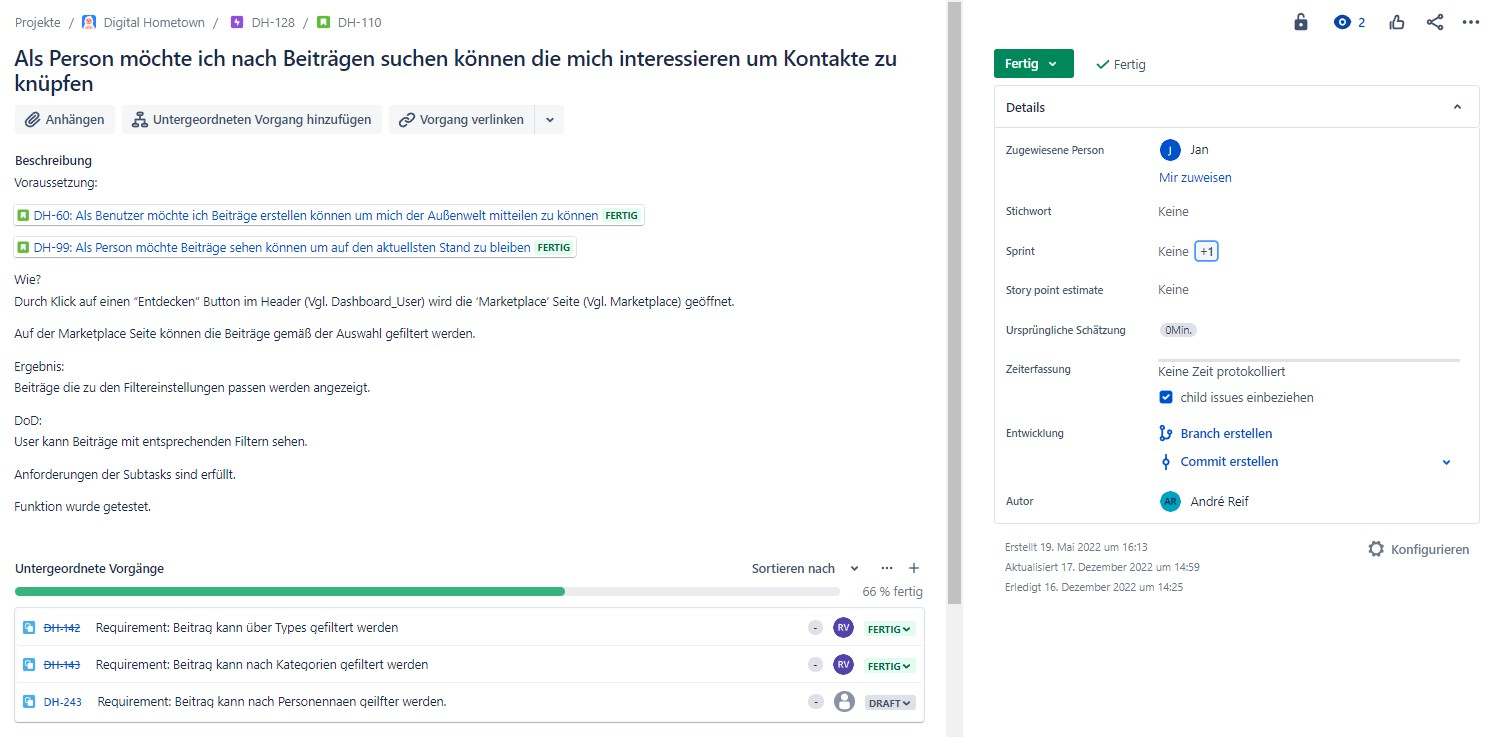
\includegraphics[width=0.6\textwidth]{figures/andre/jiratask.jpg}
    \caption{Beispiel für einen Task im JIRA}
    \label{fig:jiratask}
\end{figure}

Einzelne Tasks können in sog. Epics geclustert werden, um so die Aufgaben und langfristige Planung besser strukturieren zu können. Im Folgenden ist eine Übersicht der Epics innerhalb des Projekts sowie deren Fortschritt zu sehen.

\begin{figure}[ht!]
    \centering
    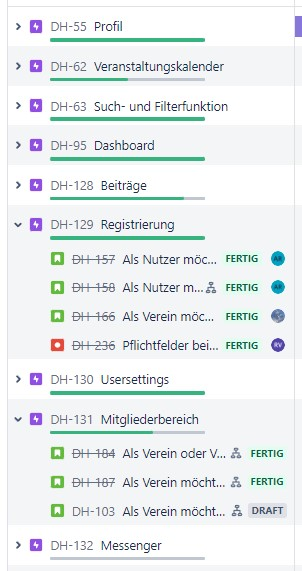
\includegraphics[width=0.6\textwidth]{figures/andre/epicsdesprojekts.jpg}
    \caption{Epic Übersicht des Projekts}
    \label{fig:epicsdesprojekts}
\end{figure}

Für die einzelnen Tasks wurden jeweils 4 verschiedene Typen unterschieden.

\subsubsection*{User-Story}
Eine User Story beschreibt eine neue Nutzeranforderung, also ein Feature, dass umgesetzt werden muss das der Benutzer die entsprechende Tätigkeit ausführen kann. Diese werden per Definition nach dem folgenden Prinzip geschrieben:

Als Nutzer möchte ich \textbf{<Auszuführende Tätigkeit>} um \textbf{<Vorteil oder Intention der ausgeführten Tätigkeit>}.

Eine User Story hat den Folgenden Aufbau:
\begin{itemize}
    \item \textbf{Titel} User Story nach Definition.
    \item \textbf{Wie?} Kurze Beschreibung wie die Funktion umgesetzt werden soll.
    \item \textbf{Ergebnis?} Beschreibung was passiert, wenn die Funktion ausgeführt wird.
    \item \textbf{DoD} Definition of Done, also eine Definition, wann der Task als erledigt gilt.
\end{itemize}

\subsubsection*{Sub-Task}
Sub-Tasks werden in der Regel dazu verwendet, um besonders aufwendige User Stories und Tasks in kleinere Arbeitseinheiten zu unterteilen. Für Digital Home Town wurden die Sub-Tasks verwendet, um Task-spezifische Anforderungen zu dokumentieren und hervorzuheben. 
\subsubsection*{Functional-Task}
Für unterstützende Arbeiten, die nicht direkt mit der Entwicklung der Plattform in Verbindung stehen, wurden sog. Functional Tasks eingeführt. Diese sind in der Regel nicht näher definiert oder Beschrieben und sind Anhand des Titels nachvollziehbar. 

\begin{figure}[ht!]
    \centering
    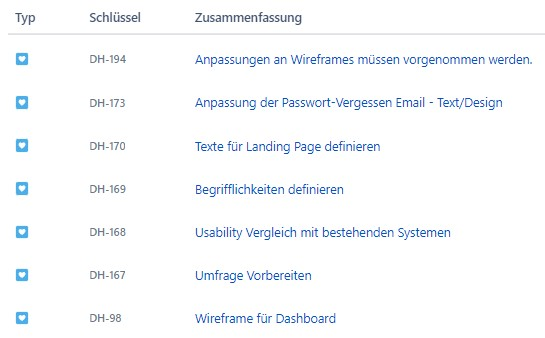
\includegraphics[width=0.6\textwidth]{figures/andre/functionaltasks.jpg}
    \caption{Beispiele für Functional Tasks}
    \label{fig:functionaltasks}
\end{figure}

\subsubsection*{Bug}
Ein Bug stellt einen gefundenen Fehler auf der Plattform da. Dieser spiegelt sowohl einen Fehlerbericht als auch einen neuen Arbeitsauftrag dar. Innerhalb des Entwicklerteams war es üblich, dass zumeist der Verursacher des Bugs auch für dessen Behebung verantwortlich war. Ein Bug durchläuft allerdings denselben Arbeitsablauf wie eine User-Story und nach den gleichen Standards getestet.

\begin{figure}[ht!]
    \centering
    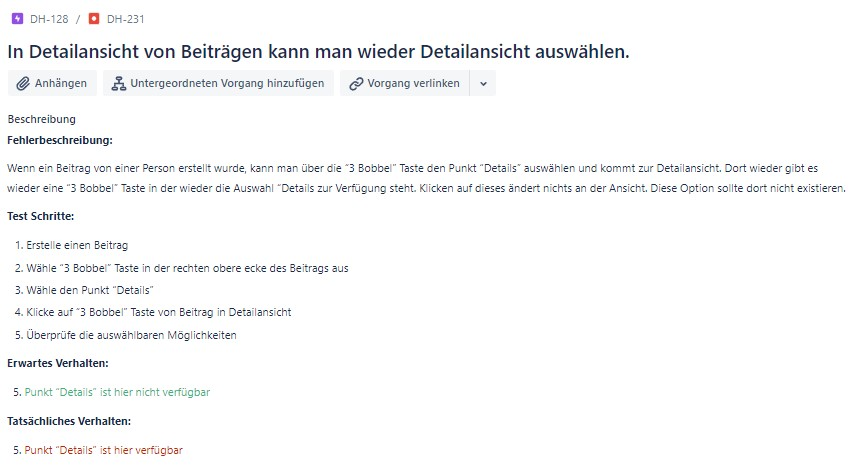
\includegraphics[width=0.6\textwidth]{figures/andre/bugticket.jpg}
    \caption{Beispiel für ein Bug Ticket}
    \label{fig:bugticket}
\end{figure}

Ein Bug besteht in der Regel aus:

\begin{itemize}
    \item \textbf{Titel} Kurze Beschreibung des Fehlers
    \item \textbf{Beschreibung} Detaillierte Beschreibung des Fehlers und des Fehlerhergangs
    \item \textbf{Test Schritte} Schritt-für-Schritt Angaben über den Ablauf des Tests
    \item \textbf{Verhalten} Erwartetes und Tatsächliches Verhalten
\end{itemize}

\subsubsection{Arbeitsablauf}
In der folgenden Abbildung ist der Allgemeine Arbeitsablauf für ein einzelnes JIRA Ticket zu sehen.

\begin{figure}[h!]
    \centering
    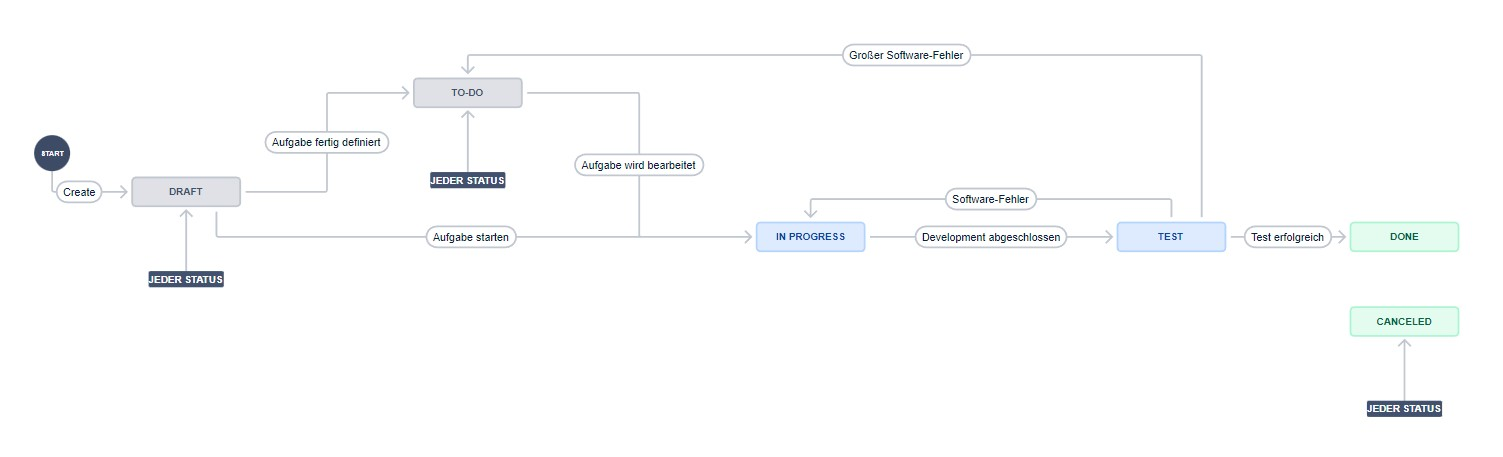
\includegraphics[width=0.6\textwidth]{figures/andre/workflow.jpg}
    \caption{Darstellung des Ablaufs eines einzelnen JIRA Tickets}
    \label{fig:workflow}
\end{figure}

Ein einzelner Task wurde zunächst mit dem Status „Draft“ erstellt. Dies wurde im Allgemeinen so interpretiert, dass das Ticket zwar angelegt wurde, jedoch nicht vom Team so akzeptiert wurde, dass jeder die Aufgabe verstanden hat. Dies wurde bei der Sprint Planung bzw. dem Task Refinement während der Planung Besprochen, ggf. angepasst, und dann festgelegt. 

Nachdem ein Task den Status „ToDo“ erhält, kann dieser in einem Sprint eingeplant und entsprechend bearbeitet werden. Der Status wechselt demnach zu „In Progress“. 

Nach der Bearbeitung wird ein Ticket mit Hilfe des Flags „Test“ zum Testen freigegeben. Das Bedeutet der Code läuft in der Entwicklungsumgebung und kann von einem Tester bearbeitet werden. Ob im Fehlerfall ein Task zurück in den Status „ToDo“ oder „In Progress“ versetzt wurde, lag in der Schwere des Fehlers und im Ermessen des jeweiligen Testers. Falls der Test erfolgreich war, wurde der Task auf den Status „Done“ verschoben und war somit abgearbeitet.

Aufgrund sich ändernder Anforderungen wurde später der „Canceled“ Staus eingeführt, um ggf. bereits begonnene Tasks abbrechen zu können.

Dieser Ablauf gilt in der Regel für jede User Story sowie jeden Bug. Die Stati „Draft“ und „Test“ hatten für Functional Tasks und Sub Tasks jedoch keine tiefergehende Bedeutung und konnten einfach übersprungen werden.

\subsection{Sprint Planning mit JIRA}
Die Sprints wurden in der Regel vorausgeplant. Dabei galt die Regel: der nächste Sprint steht am Ende des aktuellsten Sprints weitestgehend fest, der übernächste Sprint ist zu 50\% geplant. 

Während der Planungsmeetings wurden die geplanten Tasks und Bugs besprochen und auf deren Umsetzbarkeit und Priorität geprüft. Aufgrund der un-terschiedlichen Kenntnisse und Fertigkeiten der Entwickler war es jedoch schwierig den Aufwand einzelner Tasks verallgemeinert für das gesamte Entwicklungsteam einzuschätzen. Zuzüglich dazu mussten Urlaubs- und Abwesenheitszeiten bei der Planung berücksichtigt werden, sodass die definierten Sprint Ziele auch erreicht werden konnten.

\begin{figure}[h!]
    \centering
    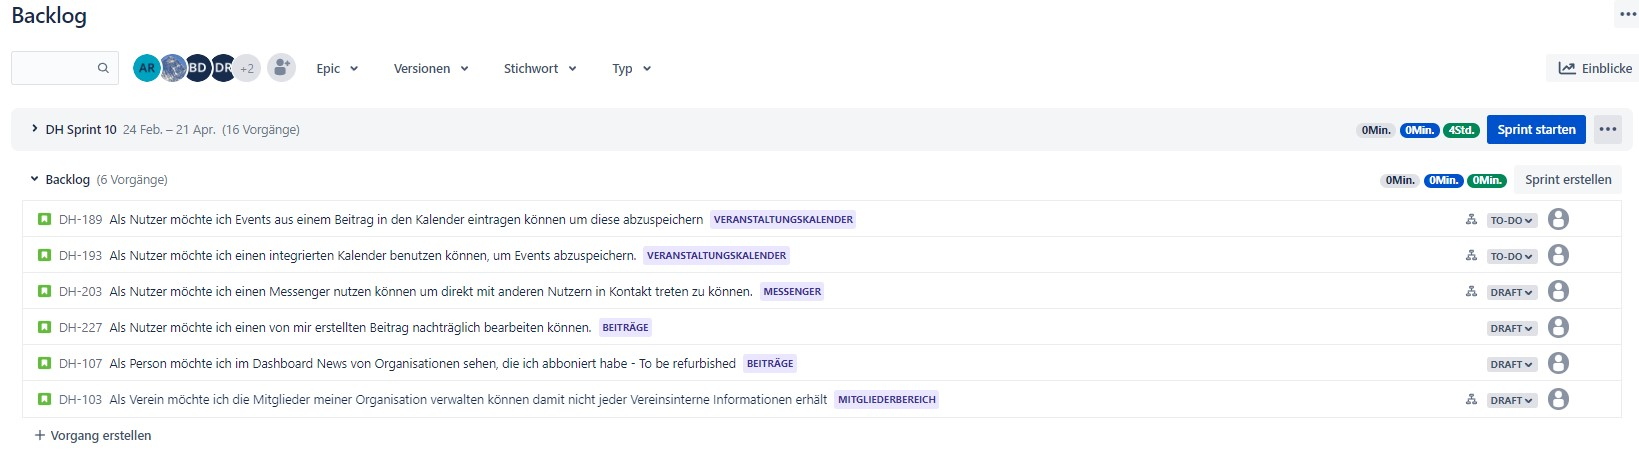
\includegraphics[width=0.6\textwidth]{figures/andre/jirabacklog.jpg}
    \caption{Backlog Funktion im JIRA}
    \label{fig:jirabacklog}
\end{figure}

Zur Planung der Sprints wurde die in der obigen Abbildung zu sehende Backlog Funktion verwendet. Hier sind zum sowohl die nicht geplanten Tasks zu sehen als auch die einem Sprint bereits zugeordnetem Task und können auch bei Bedarf entsprechend umgeplant werden. So war es nicht unüblich, dass nachdem das Sprintziel bereits vor dem Ende des Sprints erreicht wurde, noch offene Bugs oder kleinere Functional Tasks dem Sprint hinzugefügt und abgearbeitet wurden. Zum Sprintende begonnene Arbeitsaufträge wurden grundsätzlich in den nachfolgenden Sprint verschoben und fertiggestellt.

\subsubsection{User Story Map}
Als weiteres Tool zur Projektplanung wurde der Ansatz des sogenannten User Story Mapping verwendet. Per Definition ist eine User Story Map eine Technik zur Visualisierung von Benutzeranforderungen und -funktionen in einer hierarchischen Struktur.

\begin{figure}[h!]
    \centering
    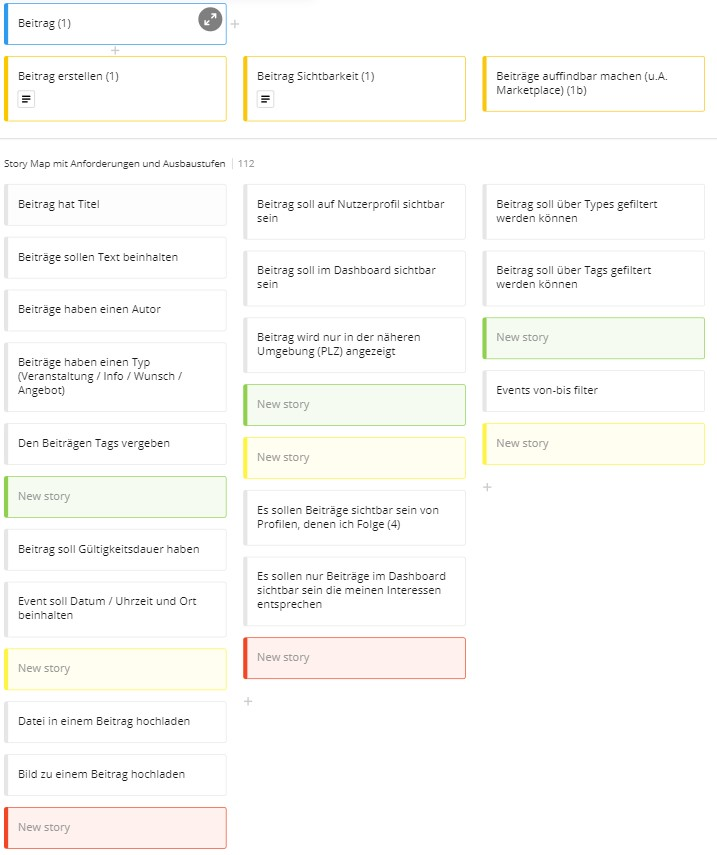
\includegraphics[width=0.6\textwidth]{figures/andre/userstorymap.jpg}
    \caption{Beiträge in der User Story Map}
    \label{fig:userstorymap}
\end{figure}

In der obigen Abbildung ist die User Story Map für einige Features der Beiträge zu finden. So gibt es zur User Story „Als Nutzer möchte ich einen Beitrag erstellen können um mich der Community mitteilen zu können“ verschiedene Anforderungen. Diese stehen unterhalb des jeweils gelben Blocks. 

Die Anforderungen jeweils wurden dann in 3 Iterationsstufen Priorisiert:

\begin{itemize}
    \item \textbf{Bis Grün} Minimum viable product, also die Minimalanforderungen die Umgesetzt werden sollen
    \item \textbf{Bis Gelb} Nice-to-Have, Anforderungen die umgesetzt werden sollen, aber nicht hoch Priorisiert werden
    \item \textbf{Bis Rot} Wird implementiert falls genügend Zeit dafür da ist
\end{itemize}

Aus dieser Map wurden dann die einzelnen User Story Tasks im JIRA angelegt und entsprechend in den Sprints verplant.